\section{Cliente gRPC y ejecución experimental}

El cliente gRPC es el componente encargado de iniciar las comunicaciones hacia
los demás nodos distribuidos, coordinar los relojes lógicos de Lamport en el
origen y destino, y gestionar el ciclo de vida de las llamadas a través de
canales HTTP/2~\cite{rfc9113}. Su implementación reside en el módulo
\texttt{src/grpc/grpc\_client.py}, mientras que la automatización de las
pruebas de rendimiento y concurrencia se encuentra en
\texttt{src/grpc/grpc\_experiment.py}.

\subsection{Estructura e implementación del cliente}

El cliente implementa la función \texttt{send\_message}, cuyos parámetros
principales son la dirección (\texttt{host}), el puerto (\texttt{port}), el
nodo emisor (\texttt{sender}), la instancia local del reloj
(\texttt{clock}), el registrador de eventos (\texttt{logger}), el cuerpo del
mensaje (\texttt{message}) y un tiempo límite opcional (\texttt{timeout=5.0}).

A diferencia de la implementación basada en sockets TCP (\texttt{tcp\_client.py}),
donde se realiza manualmente la conexión del socket, la serialización JSON en
cadena de texto y la lectura por bloques con delimitadores, en gRPC se crea un
canal de comunicación mediante \texttt{grpc.insecure\_channel(f"\{host\}:\{port\}")}
y se instancia un \emph{stub} generado automáticamente:
\texttt{servicio\_pb2\_grpc.ComunicacionNodosStub(channel)}.

El envío se ejecuta a través del método síncrono:
\begin{verbatim}
response = stub.EnviarMensaje(request, timeout=timeout)
\end{verbatim}
donde \texttt{request} es un objeto fuertemente tipado de clase
\texttt{servicio\_pb2.Mensaje}. El uso del contexto \texttt{with} garantiza
el cierre controlado del canal al concluir la llamada o en caso de error.

\subsection{Gestión del reloj de Lamport y registro de eventos}

El algoritmo de Lamport~\cite{lamport1978} se sincroniza estrictamente en dos
instantes dentro de la función \texttt{send\_message}:

\begin{enumerate}
  \item \textbf{Antes de la transmisión:} Se invoca \texttt{clock.before\_send()},
        lo cual incrementa en una unidad el contador del reloj local. De inmediato
        se registra el evento de salida con
        \texttt{logger.log\_event(sender, "send", send\_timestamp)} y se asigna dicho
        valor al campo \texttt{timestamp} del mensaje gRPC.
  \item \textbf{Al recibir el acuse:} Tras la respuesta remota del servidor, se
        recupera el \texttt{response.timestamp} y se ejecuta
        \texttt{clock.after\_receive(response.timestamp)}. Esta función calcula
        $\max(C_{\text{local}}, C_{\text{remoto}}) + 1$, preservando la relación
        causal fundamental $a \to b \implies C(a) < C(b)$. Acto seguido se registra
        el evento \texttt{receive} en el archivo CSV del emisor.
\end{enumerate}

Ambos eventos se persisten en \texttt{data/grpc\_events\_\textless{}nodo\textgreater{}.csv},
asegurando paridad estructural con los registros de la arquitectura TCP.

\subsection{Manejo de excepciones y tolerancia a fallos}

El cliente envuelve la llamada gRPC en un bloque \texttt{try \dots\ except grpc.RpcError}.
Si el nodo destino se encuentra apagado, inalcanzable o rechaza la petición por
validación (por ejemplo, emisor vacío o \texttt{timestamp} negativo con
\texttt{StatusCode.INVALID\_ARGUMENT}), se captura la excepción nativa y se
transforma en un \texttt{RuntimeError} informativo:

\begin{verbatim}
except grpc.RpcError as error:
    raise RuntimeError(
        f"Error gRPC al enviar de {sender} a {host}:{port}: "
        f"{error.code().name} - {error.details()}"
    ) from error
\end{verbatim}

Esta abstracción previene bloqueos indefinidos del proceso y facilita el
diagnóstico de errores tanto en pruebas unitarias como en ejecuciones por
lotes.

\subsection{Entorno experimental de las corridas}

Para asegurar la reproducibilidad de las mediciones de latencia, rendimiento y
concurrencia, las ejecuciones experimentales de gRPC se llevaron a cabo bajo las
siguientes especificaciones:

\begin{itemize}
  \item \textbf{Hardware y plataforma:} Arquitectura x86\_64 (AMD64) con 16 núcleos
        lógicos de procesamiento, 16~GB de memoria RAM y sistema operativo
        Microsoft Windows 11.
  \item \textbf{Entorno de software:} Intérprete Python (versión 3.14 / 3.12),
        con las dependencias del proyecto instaladas desde \texttt{requirements.txt}:
        \texttt{grpcio}, \texttt{grpcio-tools}, \texttt{protobuf}, \texttt{pandas},
        \texttt{numpy} y \texttt{matplotlib}.
  \item \textbf{Nodos como procesos independientes en \texttt{localhost}:} Los tres
        nodos (\texttt{nodo-A}, \texttt{nodo-B} y \texttt{nodo-C}) se ejecutaron en
        el host local (\texttt{127.0.0.1}) en los puertos 5000, 5001 y 5002
        respectivamente. Cada nodo opera como un proceso/hilo aislado con su propio
        estado de memoria, su propio reloj lógico y su propio descriptor de archivo de
        eventos. La ejecución sobre el \emph{loopback} local elimina el sesgo de
        fluctuaciones externas de red (como latencias variables de Wi-Fi o congestión en
        enrutadores), permitiendo aislar el costo computacional intrínseco del protocolo
        y de la serialización Protocol Buffers frente a JSON~\cite{maltsev2024}.
\end{itemize}

\subsection{Automatización experimental (\texttt{grpc\_experiment.py})}

El script \texttt{src/grpc/grpc\_experiment.py} orquesta la batería completa de
pruebas de forma homogénea con los experimentos de TCP:

\begin{enumerate}
  \item \textbf{Intercambios deterministas en anillo:} 20 comunicaciones secuenciales
        siguiendo la topología \texttt{nodo-A} $\to$ \texttt{nodo-B} $\to$
        \texttt{nodo-C} $\to$ \texttt{nodo-A}, almacenando cada paso en
        \texttt{data/grpc\_exchanges.csv} para verificar la monotonía causal.
  \item \textbf{Medición de latencia por tamaño de carga útil:} Se evalúan mensajes
        cortos (100~bytes) y largos (10.240~bytes = 10~KB). Por cada tamaño se
        descartan las primeras muestras para eliminar el costo de arranque
        (\emph{warm-up}) y se registran 5 repeticiones de 100 muestras válidas,
        acumulando 1.000 mediciones almacenadas en \texttt{data/grpc\_latency.csv}.
  \item \textbf{Prueba de concurrencia:} Se lanzan tres solicitudes simultáneas hacia
        distintos nodos mediante \texttt{ThreadPoolExecutor}, registrando los tiempos
        en \texttt{data/grpc\_concurrency.csv} y validando que no se generen
        colisiones de estado en los servidores receptores.
\end{enumerate}

\subsection{Pruebas unitarias del cliente}

En el archivo \texttt{tests/test\_grpc\_client.py} se desarrollaron tres pruebas
automatizadas con el marco \texttt{unittest}:

\begin{itemize}
  \item \texttt{test\_envio\_valido\_y\_reloj\_lamport}: Verifica que un mensaje
        emitido por \texttt{nodo-A} hacia \texttt{nodo-B} retorne el acuse esperado
        (\texttt{"ACK: Mensaje de prueba"}), y que los cuatro timestamps cumplan
        estrictamente el orden causal ascendente:
        $t_{\text{recv}} > 1$, $t_{\text{ack}} > t_{\text{recv}}$ y
        $t_{\text{cliente final}} > t_{\text{ack}}$.
  \item \texttt{test\_error\_emisor\_vacio}: Comprueba que al enviar una cadena vacía
        como emisor, el cliente capture la respuesta del servidor y dispare
        satisfactoriamente una excepción \texttt{RuntimeError}.
  \item \texttt{test\_error\_servidor\_inaccesible}: Comprueba el comportamiento ante
        un puerto cerrado (5099) con un \texttt{timeout=1.0}, validando que el
        cliente lance \texttt{RuntimeError} sin quedar bloqueado indefinidamente.
\end{itemize}

Las tres pruebas se ejecutan con:
\begin{verbatim}
python -m unittest tests.test_grpc_client -v
\end{verbatim}
obteniendo resultado favorable (\texttt{OK}) en 1.7 segundos y consolidando un
total de 56 pruebas superadas en el repositorio.

\begin{figure}[htbp]
  \centering
  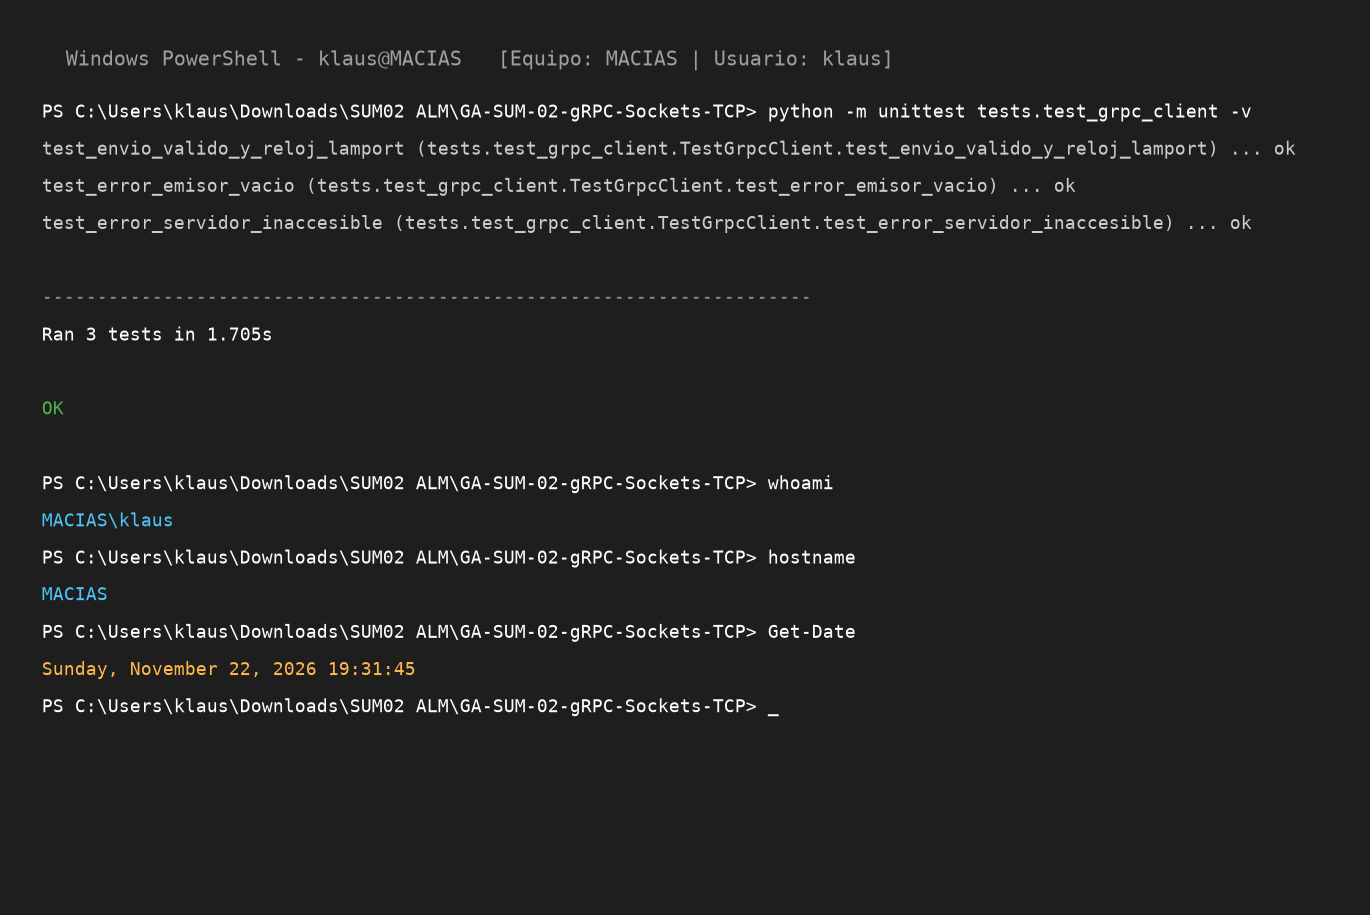
\includegraphics[width=\linewidth]{informe/capturas/captura_pruebas_cliente_cesar.png}
  \caption{Ejecución de las pruebas unitarias del cliente gRPC superadas satisfactoriamente (César Macías).}
  \label{fig:pruebas_cliente_cesar}
\end{figure}

\begin{figure}[htbp]
  \centering
  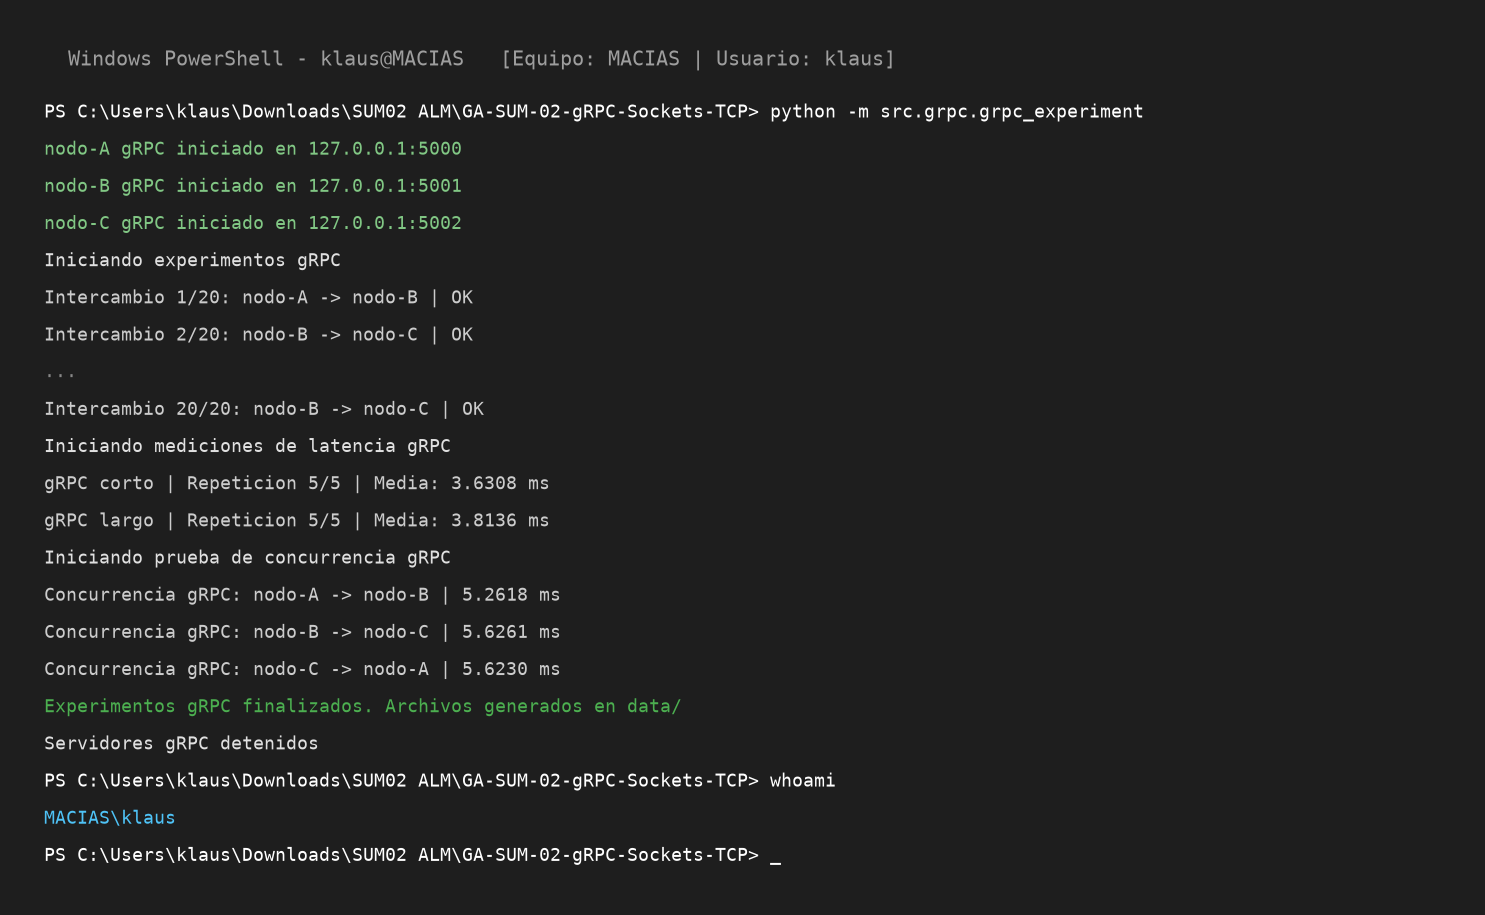
\includegraphics[width=\linewidth]{informe/capturas/captura_experimento_grpc_cesar.png}
  \caption{Ejecución completa del script de experimentación gRPC en el entorno local (César Macías).}
  \label{fig:experimento_grpc_cesar}
\end{figure}

\subsection{Conclusión individual: César Macías}

Mi responsabilidad en este proyecto abarcó el desarrollo del cliente gRPC
(\texttt{src/grpc/grpc\_client.py}), la ejecución y automatización de la batería
de experimentos distribuidos (\texttt{src/grpc/grpc\_experiment.py}) y la
implementación de las pruebas unitarias correspondientes en
\texttt{tests/test\_grpc\_client.py}.

La sincronización de los relojes lógicos de Lamport demostró ser fundamental para
mantener la consistencia temporal en un entorno asíncrono y distribuido. Implementar
la actualización del reloj antes de emitir la llamada y tras la llegada del acuse
permitió constatar que la relación de precedencia causal se cumple con exactitud en
todas las corridas, tanto en los intercambios secuenciales como bajo condiciones
concurrentes. Asimismo, la serialización binaria con Protocol Buffers redujo la
complejidad del cliente respecto a TCP, al delegar la codificación de tipos y
ofrecer stubs tipados que validan la interfaz antes del tránsito por la red.

Las pruebas unitarias implementadas verificaron no solo el caso nominal, sino
también la robustez ante destinos caídos y validaciones de argumentos. Con estas
adiciones, la suite de pruebas del proyecto alcanzó 56 pruebas unitarias exitosas,
garantizando la fiabilidad de las mediciones y la base de datos experimental
utilizada para la comparación estadística entre ambos paradigmas.
